% -------------------------------------------------------------------------------------------------
% Creation date: 08May2018
% Author: Anthony Williams
% This is a latex template designed to mimic to HVTN PT Reports.
% It's intended to be used with Rmarkdown to generate single-document reports.

% Modification log:
% 27 May 2022, Namita Trikannad: 
% Added hyperref code to enable TOC linking 
% Added CSL referencing to make the TOC linking work correctly 

% 29 August 2022, Namita Trikannad: 
% Added hyperref code to enable working links in the Table of Contents (TOC), List of Tables (LOT) and Figures (LOF).  

% 30 August 2022, Namita Trikannad:
% Added a new command to remove content numbering in TOC, LOT, and LOF

% 2 September 2022, Namita Trikannad:
% Added TOC, LOT, and LOF under if commands to display based on user input in the Skeleton YAML 

% 7 October 2022, Namita Trikannad: 
% Added 'floatrow' code to enable placement of figure captions on top, and code to render kable/kableExtra tables when using 'floatrow' instead of 'float'. 
% Notes: : 'floatrow' and 'float' are incompatible. Do not load them together, as one may overwrite or silence the other. 'float' is required to properly place and format kable and kableExtra tables rendered via markdown. If using 'floatrow' (required for figure captions to be placed on top), mute loading of 'float', and use the code under "'floatrow' code section" to render kable/kableExtra tables. If using 'float', mute loading 'floatrow' and the sections using floatrow code. 
% -------------------------------------------------------------------------------------------------

\documentclass[12pt]{article}
% Current PT report margins are as follows:
% Top = 1in, bottom = 0.5in, left/right = 0.75in.
% Title page: Top/bottom Logo goes another 0.5in,
% Other pages: footer = addition 0.25 in, header = 0.5 in
\usepackage[margin=0.75in, top=0.5in, bottom=1in, includeheadfoot]{geometry} % for margins
\usepackage[dvipsnames]{xcolor} % for line colors, argument for using more color names
\usepackage{colortbl} % for coloring table lines
\usepackage{fancyhdr} % for headers and footers
\usepackage{graphicx} % for images
\usepackage{fontspec} % to use different fonts
\IfFontExistsTF{Arial}{\setmainfont{Arial}}{\setmainfont{Open Sans}}
\usepackage{lastpage} % For page number
\usepackage{pdflscape} % for landscape pages
\usepackage[absolute]{textpos} % for rotating landscape header/footers
\usepackage{longtable} % for longtables
\usepackage{booktabs} % for \toprule
\usepackage{caption} % for manipulating table captions.
\usepackage{hyphenat} % handle hyphens correctly, keeps from running into margins
\usepackage{tabu}
\usepackage{threeparttable} % for long footnotes
\usepackage{threeparttablex}
\usepackage[citestyle=authoryear-comp,natbib=true]{biblatex}
\usepackage{titlesec}
\usepackage{hyperref} % for TOC and URLs in bibliography
\usepackage{floatrow} % place figure captions on top; do not load with 'float'
% \usepackage{float} % enable if not using floatrow

\usepackage{booktabs}
\usepackage{longtable}
\usepackage{array}
\usepackage{multirow}
\usepackage{wrapfig}
\usepackage{float}
\usepackage{colortbl}
\usepackage{pdflscape}
\usepackage{tabu}
\usepackage{threeparttable}
\usepackage{threeparttablex}
\usepackage[normalem]{ulem}
\usepackage{makecell}
\usepackage{xcolor}
% 

% Add this to handle CSLReference dependency introduced in Pandoc v2.8+
\newlength{\cslhangindent}
\setlength{\cslhangindent}{1.5em}
\newenvironment{CSLReferences}%
  {}%
  {\par}

\bibliography{bibliography.bib}

\setlength\parindent{0pt} % no paragraph indentation
\setlength{\parskip}{12pt} % blank line between each paragraph

% Adding referencing code for TOC links to work

\hypersetup{
  colorlinks   = true, %Colours links instead of ugly boxes
  urlcolor     = blue, %Colour for external hyperlinks
  linkcolor    = blue, %Colour of internal links
  citecolor   = gray %Colour of citations
}

% Specify captions located above figures using 'floatrow' package. Disable if not desired or need to use 'float' package.

\floatsetup[figure]{capposition=top, captionskip=0cm} %`capposition' places the fig.cap captions as titles on the top; 'captionskip' is the white space between caption and figure
\floatplacement{figure}{H} % Figure position according to the code flow.
\floatplacement{table}{H} % Table position according to the code flow.
\floatplacement{longtable}{H} % Table position according to the code flow.
\floatsetup[longtable]{margins=centering} % Longtable tables centered.
\captionsetup[longtable]{justification=raggedright, singlelinecheck=false}
\captionsetup[table]{justification=raggedright, singlelinecheck=false}


% ------------------------------------------------------------------------------
% Define commands here
% ------------------------------------------------------------------------------
% This avoids a tightlist pandoc error
\providecommand{\tightlist}{%
  \setlength{\itemsep}{0pt}\setlength{\parskip}{0pt}}
  
% NT: Removing content numbering in toc, lot, and lof
\newcommand{\removecontentnumber}{%
\let\oldnumberline\numberline
\renewcommand{\numberline}[1]{\oldnumberline{}}
\renewcommand{\numberline}[1]{\hspace*{-0.5em}}
}


% This is for vertical spacing between memo header table
\renewcommand{\arraystretch}{1.5}

% This command is basically hrullfill, but makes the width dynamic.
% For use with the first footer rule, since it's different than the other header/footer rules
\newcommand*\varhrulefill[1][2pt]{\leavevmode\leaders\hrule height#1\hfill\kern0pt}

% This is for resetting normal page margins from within the Rmarkdown document.
% Otherwise we can only change geometry before or after the Rmd text.
\newcommand{\memogeo}{\newgeometry{margin=0.75in, top=0.5in, includeheadfoot}}
\newcommand{\tlfgeo}{\newgeometry{margin=0.25in, top=0in, includeheadfoot}}
\newcommand{\figmargins}{%
  %\newgeometry{margin=-1.5in, bottom=0in, left=0in, includeheadfoot}
  \newgeometry{top=0.12in, bottom=0.12in, left=0in, right=0.2in, includeheadfoot}
}

% These commands apply the geometries define above anywhere within the Rmd
\newcommand{\memoformat}{%
  \memogeo
  \pagestyle{memopage}
}

\newcommand{\tlf}{%
  \tlfgeo
  \pagestyle{tlfpage}
}

% Commands for creating landscape pages. Eventually we can define a style for landscape pages
% Hopefully that will allow us to put use headers/footers/page numbers
\newcommand{\blandscape}{\begin{landscape}\pagestyle{landscapepage}}
\newcommand{\elandscape}{\end{landscape}}

% Header and Footer -------

% The bulk of the HVTN PT report format is in the headers and footers. Specifically,
% the first pages header and footer images. Here we create two page styles, for the
% first and subsequent pages, respectively.

% First page style
\fancypagestyle{memohead}{%

  \fancyhf{}% Clear all headers/footers

  \fancyhead[L]{\fontsize{20}{12} \selectfont \bf{MEMORANDUM}}% Header
  \renewcommand{\headrulewidth}{2pt}% 2pt header rule
  \renewcommand{\headrule}{\hbox to\headwidth{%
    \color{Tan}\leaders\hrule height \headrulewidth\hfill}}

  \renewcommand{\footrulewidth}{0pt} % Remove default foot rule
  % Footer is actually a combination of left, center, and right footers.
  \fancyfoot[LE,LO]{~\\{\color{Tan}\varhrulefill}\\~\\\fontsize{10}{12} \selectfont 1100 Fairview Ave N - LE-400 - PO Box 19024 - Seattle, WA 98109-1024 - (206) 667-7000 - (206) 667-4812 Fax}% Footer}
  \fancyfoot[CE,CO]{
\includegraphics[width=2in]{resources/fhcc.jpg}\\{\color{Tan}\varhrulefill}\\~}
  \fancyfoot[RE,RO]{~\\{\color{Tan}\varhrulefill}\\\fontsize{10}{12} \selectfont Page \thepage\ of \pageref{LastPage}}

  % Add figures to memo header
  \chead{
\includegraphics[width=1.5in]{resources/hvtn.jpg}}
  \rhead{
\includegraphics[width=2in]{resources/scharp.jpg}}
} % end of fancypagestyle{memohead}

% Subsequenct page styles
\fancypagestyle{memopage}{%

  % less spacing around memo section headers
  \titlespacing*{\subsection}
  {0pt}{0pt}{0pt}

  \fancyhf{}% Clear all headers/footers

  \fancyhead[R]{\fontsize{20}{12} \selectfont \bf{Memorandum, continued}}

  \fancyfoot[R]{\fontsize{10}{12} \selectfont Page \thepage\ of \pageref{LastPage}}
 \fancyfoot[C]{\fontsize{10}{12} \selectfont ~ \\ \fontsize{10}{12} \selectfont 1100 Fairview Ave N - LE-400 - PO Box 19024 - Seattle, WA 98109-1024 - (206) 667-7000 - (206) 667-4812 Fax}% Footer

  % Header line
  \renewcommand{\headrulewidth}{2pt}% 2pt header rule
  \renewcommand{\headrule}{\hbox to\headwidth{%
    \color{Tan}\leaders\hrule height \headrulewidth\hfill}}

  % Footer line
  \renewcommand{\footrulewidth}{2pt}% 2pt footer rule
  \renewcommand{\footrule}{\hbox to\headwidth{%
    \color{Tan}\leaders\hrule height \footrulewidth\hfill}}
} % end of fancypagestyle{normalpage}

\fancypagestyle{tlfpage}{%
  \fancyhf{}% clear all headers/footers
  % Header line
  \renewcommand{\headrulewidth}{2pt}% 2pt header rule
  % Footer line
  \renewcommand{\footrulewidth}{2pt}% 2pt footer rule
   \renewcommand{\footrulewidth}{0pt}% footer rule
  \renewcommand{\headrulewidth}{0pt}% header rule
   \fancyfoot[R]{\fontsize{10}{12} \selectfont Page \thepage\ of \pageref{LastPage}}% Footer
}

% Set footer for landscape pages. We only need the page number because these are TLFs.
\fancypagestyle{landscapepage}{%
  \fancyhf{}
  \renewcommand{\footrulewidth}{0pt}% footer rule
  \renewcommand{\headrulewidth}{0pt}% header rule
}

\setlength{\headheight}{20pt} % This adds space between the header line and body text.
\setlength{\footskip}{20pt} % this is the same for footers, but haven't figured out how it works.

%%% If debugging the template.tex file, remove these if statements!!! ------
%%% -----------------------------------------------------------------------
%This removes some shading warning when inserting code in Rmarkdown

% Remove numbered sections
\setcounter{secnumdepth}{0}

% ---------------------------------------------------------------------------

% End of premable -----

\begin{document}

\pagestyle{memopage} % Set header/footers for all pages
\thispagestyle{memohead} % Add memo header and line on first page
% Memo header table.
% Need the color statement for vertical bars, according to colortbl documentation
\vspace*{1cm} % need the * so it doesn't get deleted
\noindent\begin{tabular}{!{\color{Tan}\vline} p{0.5in} !{\color{Tan}\vline} p{6.15in} !{\color{Tan}\vline}}
  \arrayrulecolor{Tan}\hline
  \bf{Date:} & {October 14, 2024} \\
  \arrayrulecolor{Tan}\hline
  \bf{To:} & {} \\
  \arrayrulecolor{Tan}\hline
  \bf{From:} & {Chenchen Yu} \\
  \arrayrulecolor{Tan}\hline
  \bf{RE:} & {hvtnFiguers::pt\_plot() test cases} \\
  \arrayrulecolor{Tan}\hline
\end{tabular}
\renewcommand{\arraystretch}{1} % Reset row spacing

\clearpage
\memoformat % Set memo format

% NT: display toc, lot, and lof based on user input
\removecontentnumber
\tableofcontents

\removecontentnumber
\listoffigures
  
\removecontentnumber
\listoftables

\clearpage

% NT

\hypertarget{executive-summary}{%
\subsection{EXECUTIVE SUMMARY}\label{executive-summary}}

This file is used for testing the hvtnFigures package. Please download
the hvtnFigures first.
\texttt{devtools::install\_github("FredHutch/hvtnFigures",\ auth\_token\ =\ auth\_token)}

In general, all plots should meet the criteria below:

\begin{enumerate}
\def\labelenumi{\arabic{enumi}.}
\item
  Each figure should be centered in the page, no cutoffs, no overlaps,
  no misalignments.
\item
  The figure matches the description in the footnote.
\item
  The figure numbers should be continuous. Missing figure numbers
  indicate hidden bugs/errors.
\item
  No missing parts in the figures. (e.g.~the boxes are imcomplete.
  Missing borders indicate narrow space between boxes and could be
  adjusted by box.width). Page titles are shown and complete (i.e.,
  figure number and caption.)
\item
  The response summary counts match the plots.
\item
  The legends are showing the correct colors/shapes in the correct
  order.
\end{enumerate}

\hypertarget{background}{%
\subsection{BACKGROUND}\label{background}}

\memoformat 

\hypertarget{schema}{%
\subsection{SCHEMA}\label{schema}}

\begin{longtable}[]{@{}lll@{}}
\toprule\noalign{}
Column 1 & Column 2 & Column 3 \\
\midrule\noalign{}
\endhead
\bottomrule\noalign{}
\endlastfoot
1 & A & - \\
2 & B & - \\
3 & C & - \\
\end{longtable}

\hypertarget{endpoints}{%
\subsection{ENDPOINTS}\label{endpoints}}

The frequency and magnitude of binding antibody responses were measured
by the HIV-1 binding antibody multiplex assay (BAMA) from specimens
obtained at months (ie, visits ) corresponding to .

\hypertarget{lab-methods}{%
\subsection{LAB METHODS}\label{lab-methods}}

HIV-1-specific responses () against were measured on a Bio-Plex
instrument (Bio-Rad) using a standardized custom HIV-1 Luminex assay
(Tomaras et al. 2008; Haynes et al. 2012; Yates et al. 2014;
Zolla-Pazner et al. 2014; Yates et al. 2018 ). The readout was
background-subtracted mean fluorescence intensity (MFI), where
background referred to a plate level control (i.e., a blank well run on
each plate). Standard positive and negative controls were included in
each assay to ensure specificity and for maintaining consistency and
reproducibility between assays. The positive control includes an IgA
control purified polyclonal IgG from HIV subjects (HIVIG) using a
10-point standard curve (4PL fit) The negative controls were NHS (HIV-1
sero-negative human sera) and blank beads.

Samples were titrated for at the month timepoint, with an -fold dilution
series of . The readout was background-subtracted mean fluorescence
intensity (MFI), where background referred to a plate level control
(i.e., a blank well run on each plate).

Total antibody (IgA or IgG) was measured using Bio-Rad Total Antibody
analysis (on a Bio-Rad Bio-Plex instrument) for each mucosal fluid to
calculate specific activity per sample (Yates et al. 2013; Seaton et al.
2014; Archary et al. 2016).

Several criteria were used to determine if data from an assay were
acceptable and could be statistically analyzed. First, the blood draw
date must have been within the allowable visit window as determined by
the protocol. Post-acquisition samples from participants who acquired
HIV are excluded. Second, if the blank bead negative control exceeded
5,000 MFI, the sample was repeated. If the repeat value exceeded MFI,
the sample was excluded from analysis due to high background. The preset
assay criteria for sample reporting were: coefficient of variation (CV)
per duplicate values for each sample are \textless{} 20\% and \(\geq\)
50 beads counted per sample. To control for protein performance, the
preset criteria include that the positive control titration in each
assay must be within +/- 3 standard deviations of the mean for each
antigen (tracked with a Levey-Jennings plot for high MFI and Area Under
the Curve (AUC)).

Data from blood draw dates outside the allowable visit window and assay
results deemed unreliable for analysis by the lab were excluded from the
analysis. Post-infection samples from HIV-infected participants are
excluded.

\hypertarget{statistical-methods}{%
\subsection{STATISTICAL METHODS}\label{statistical-methods}}

The analysis in this report was carried out in accordance with SAP
version X.X.

Samples from post-enrollment visits were declared to have positive
responses if they met three conditions: (1) the MFI minus Blank values
were \(\geq\) antigen-specific cutoff at the dilution level (based on
the 95th percentile of baseline samples as calculated by SAS PROC
UNIVARIATE default method, and at least 100 MFI), (2) the MFI minus
Blank values were greater than 3 times the baseline (day 0) MFI minus
Blank values, and (3) the MFI values were greater than 3 times the
baseline MFI values.

Area under the titration curve (AUTC) was calculated for each sample,
isotype, and antigen using the trapezoidal rule, where the x-axis is
log10 of dilution and the y-axis is truncated Net MFI with negative
values set to 0 for the calculation. AUTC was not calculated for any
samples which were incompletely titrated, or where a dilution was
missing due to failing QC criteria. The response call described above
was derived from dilution .

Mucosal binding antibody magnitude was quantified in terms of specific
activity (SA). Here SA was defined as
MAX(0.0002,MFI-Blank*dilution/total antibody concentration), where total
antibody concentration is in . Samples from post-enrollment visits were
declared to have positive responses if they met three conditions: 1) SA
\textgreater{} 95th percentile of SA from unvaccinated samples from HVTN
protocols 076, 086, 088, 096, 097, and 205 combined, 2) MFI
\textgreater{} 100 and 3) SA \textgreater{} 3 times baseline SA. If
total antibody at baseline was missing, baseline SA was calculated as
the median SA of unvaccinated samples from 076, 086, 088, 096, 097, and
205 combined. .

Tables show positive response rates and corresponding 95\% confidence
intervals calculated by the Wilson score method (Agresti and Coull
1998), as well as summary statistics among positive responders and all
participants.

Barnard's test was used to compare response rates between treatment
groups, while the Wilcoxon rank sum test was used to compare response
magnitudes between treatment groups, among positive and negative
responders, and among the subset of positive responders.

Net MFI responses at the dilution level were used to summarize the
magnitude at a given time-point. These distributions are displayed
graphically by treatment arm. Plots include data from responders in
color and non-responders in gray, with box plots based on data from
responders superimposed on the distribution. Data points for each
participant are connected by a gray line. The mid-line of the box
denotes the median and the ends of the box denote the 25th and 75th
percentiles. The whiskers that extend from the top and bottom of the box
extend to the most extreme data points that are no more than 1.5 times
the interquartile range (i.e., height of the box) or if no value meets
this criterion, to the data extremes.

Partial magnitude-breadth (M-B) plots characterize the magnitude and
breadth of each individual plasma sample assayed against a panel of
antigens (Huang et al. 2009). Magnitude is net MFI, and breadth is the
number of antigens with positive response at a given value of net MFI
(\textgreater100). The x-axis represents the response magnitude on the
log10 scale and the y-axis represents the fraction of antigens with
response magnitude greater than the x-axis value. The antigen-specific
net MFI value of a negative responder is set to 100. Plots are
left-truncated at 2 on the log10 scale (i.e.~net MFI = 100), the lower
limit of the linear range of the BAMA assay. In addition to the
individual subject-specific curves, the group-specific curve displays
the average M-B across all subjects in that group. AUC-MB was calculated
as the area under the MB-curves over the entire range without
truncation, which is equivalent to the average of the log10 net MFI over
the panel of antigens.

\hypertarget{participant-cohort}{%
\subsection{PARTICIPANT COHORT}\label{participant-cohort}}

The study enrolled . Data available for analysis are summarized in the
table below.

\begin{longtable}[]{@{}
  >{\raggedright\arraybackslash}p{(\columnwidth - 6\tabcolsep) * \real{0.2143}}
  >{\raggedright\arraybackslash}p{(\columnwidth - 6\tabcolsep) * \real{0.1429}}
  >{\raggedright\arraybackslash}p{(\columnwidth - 6\tabcolsep) * \real{0.2619}}
  >{\raggedright\arraybackslash}p{(\columnwidth - 6\tabcolsep) * \real{0.3810}}@{}}
\toprule\noalign{}
\begin{minipage}[b]{\linewidth}\raggedright
Visit (month)
\end{minipage} & \begin{minipage}[b]{\linewidth}\raggedright
Group
\end{minipage} & \begin{minipage}[b]{\linewidth}\raggedright
Data available
\end{minipage} & \begin{minipage}[b]{\linewidth}\raggedright
Reason for unavailability
\end{minipage} \\
\midrule\noalign{}
\endhead
\bottomrule\noalign{}
\endlastfoot
10 (6.5) & P1-P4 & 9 & - \\
& T1 & 4 & 1 HIV acquisition \\
& T2 & 20 & 1 missed visit \\
\end{longtable}

\hypertarget{results}{%
\subsection{RESULTS}\label{results}}

\hypertarget{references}{%
\subsection{REFERENCES}\label{references}}

Liu Q, Li C, Wanga V, Shepherd BE. Covariate-adjusted Spearman's rank
correlation with probability-scale residuals. Biometrics. 2018
Jun;74(2):595-605.

Tay MZ, Liu P, Williams LD, et al.~Antibody-Mediated Internalization of
Infectious HIV-1 Virions Differs among Antibody Isotypes and Subclasses.
PLoS Pathog. 2016;12(8):e1005817.

Tomaras GD, Yates NL, Liu P, et al.~Initial B-cell responses to
transmitted human immunodeficiency virus type 1: virion-binding
immunoglobulin M (IgM) and IgG antibodies followed by plasma anti-gp41
antibodies with ineffective control of initial viremia. J Virol.
2008;82(24):12449-12463.

Haynes BF, Gilbert PB, McElrath MJ, et al.~Immune-correlates analysis of
an HIV-1 vaccine efficacy trial. N Engl J Med. 2012;366(14):1275-1286.

Yates NL, Liao HX, Fong Y, et al.~Vaccine-induced Env V1-V2 IgG3
correlates with lower HIV-1 infection risk and declines soon after
vaccination. Sci Transl Med. 2014;6(228):228ra39.

Zolla-Pazner S, deCamp A, Gilbert PB, et al.~Vaccine-induced IgG
antibodies to V1V2 regions of multiple HIV-1 subtypes correlate with
decreased risk of HIV-1 infection. PLoS One. 2014;9(2):e87572.

Liao HX, Bonsignori M, Alam SM, et al.~Vaccine induction of antibodies
against a structurally heterogeneous site of immune pressure within
HIV-1 envelope protein variable regions 1 and 2. Immunity.
2013;38(1):176-186.

Yates NL, deCamp AC, Korber BT, et al.~HIV-1 Envelope Glycoproteins from
Diverse Clades Differentiate Antibody Responses and Durability among
Vaccinees. J Virol. 2018;92(8):e01843-17.

\emph{SOURCE: SCHARP C:/Users/jkee2/OneDrive - Fred Hutch Cancer
Center/Documents/GitHub/hvtnFiguresTestRMD 4.3.3 14Oct24 15:35}

\tlf

\figmargins  \blandscape  \clearpage
\captionsetup[figure]{labelformat=empty, font=Large, labelfont=Large}

\begin{figure}[H]

{\centering 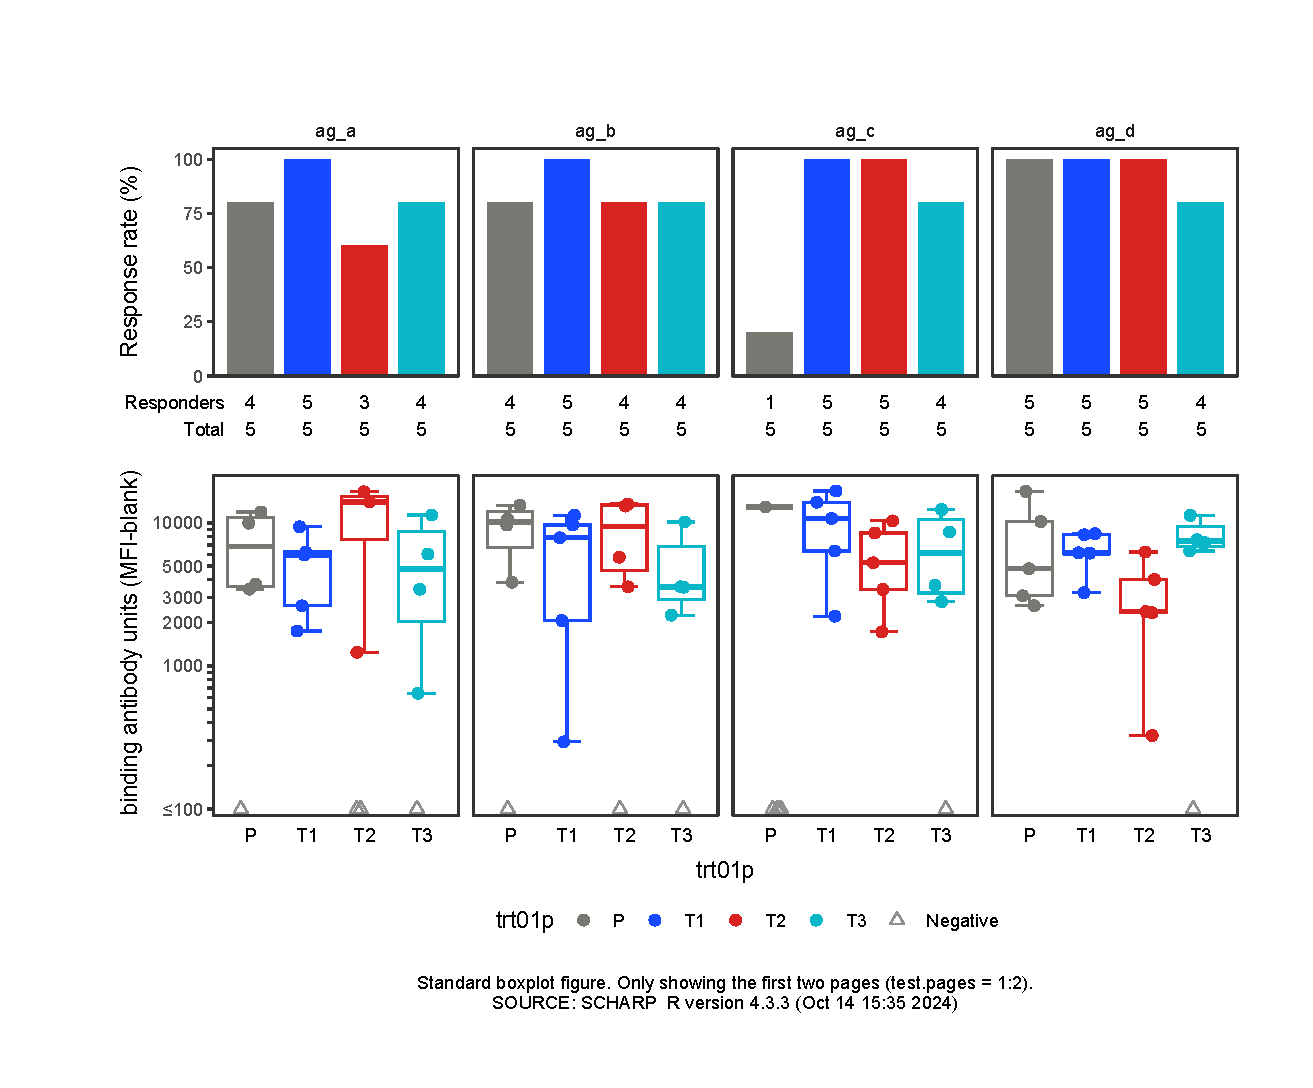
\includegraphics[width=8.75in,height=7.25in]{test_cases_files/figure-latex/unnamed-chunk-2-1} 

}

\caption[Figure 1.1 boxplot (pos. response boxplots)]{Figure 1.1 HVTN XYZ: IgA Response at Visit 5}\label{fig:unnamed-chunk-2-1}
\end{figure}
\clearpage\begin{figure}[H]

{\centering 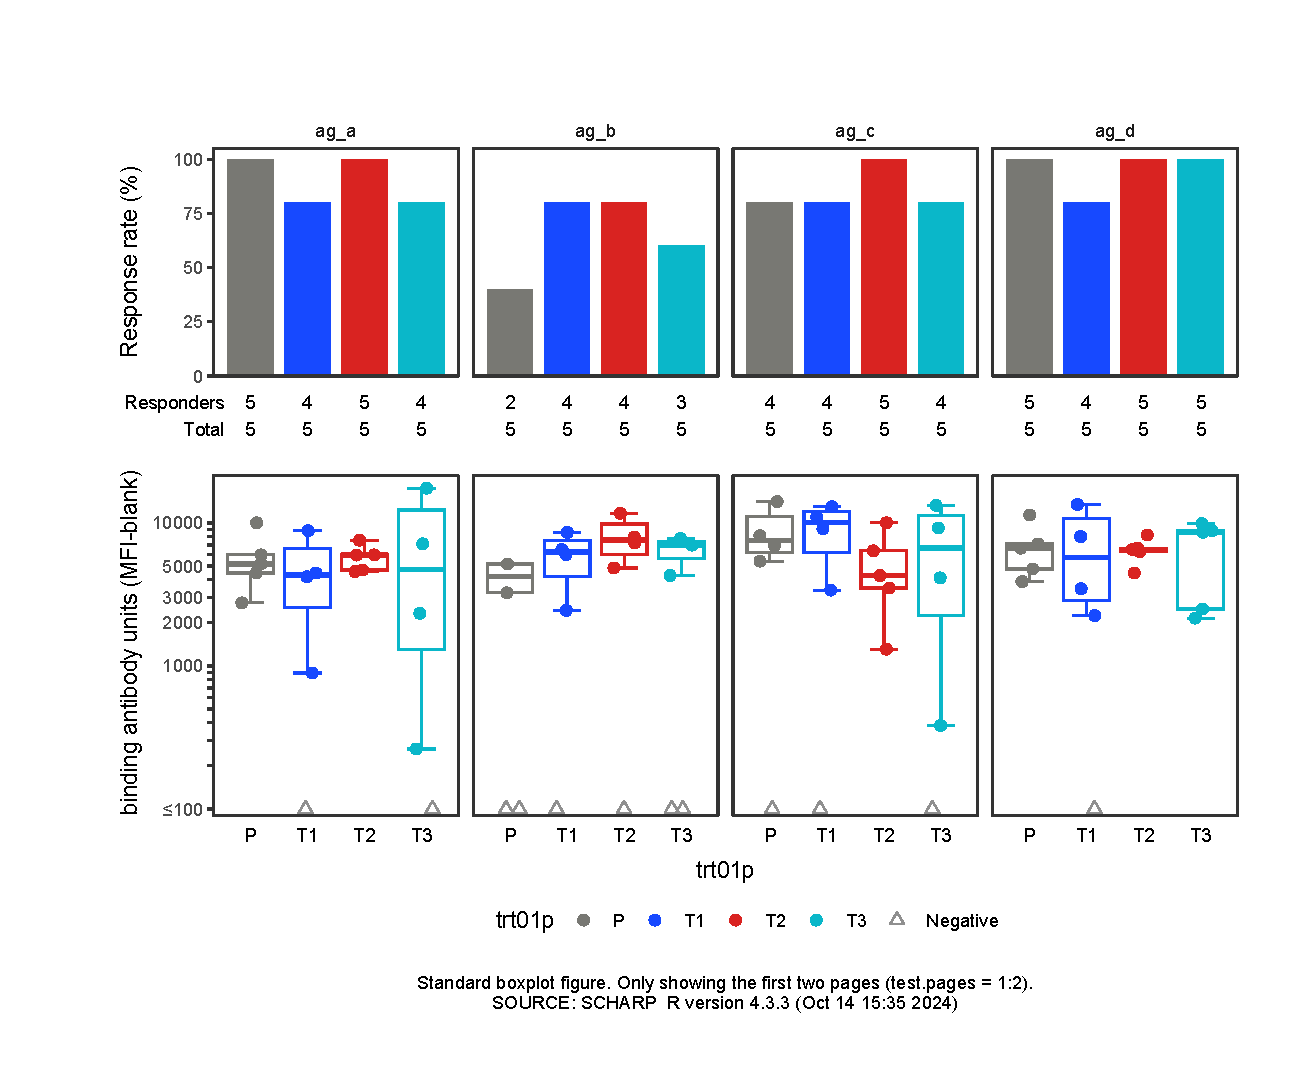
\includegraphics[width=8.75in,height=7.25in]{test_cases_files/figure-latex/unnamed-chunk-2-2} 

}

\caption[Figure 1.2 boxplot (pos. response boxplots)]{Figure 1.2 HVTN XYZ: IgA Response at Visit 7}\label{fig:unnamed-chunk-2-2}
\end{figure}
\clearpage

\begin{figure}[H]

{\centering 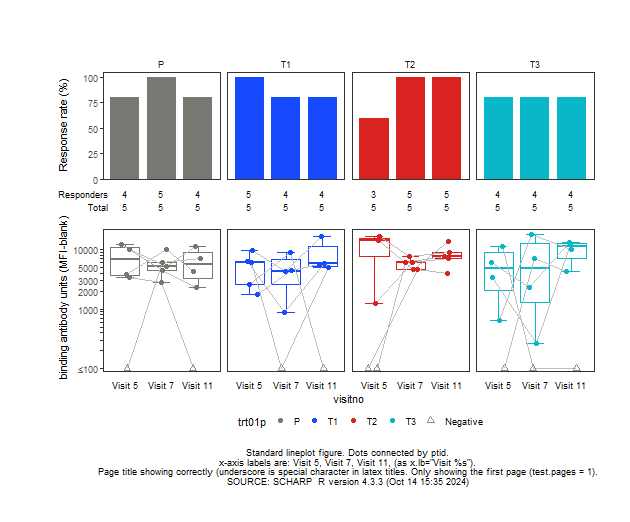
\includegraphics[width=8.75in,height=7.25in]{test_cases_files/figure-latex/unnamed-chunk-4-1} 

}

\caption[Figure 2.1 lineplot (pos. response boxplots)]{Figure 2.1 HVTN XYZ: IgA Response at Visit ag\_a}\label{fig:unnamed-chunk-4}
\end{figure}
\clearpage

\begin{figure}[H]

{\centering 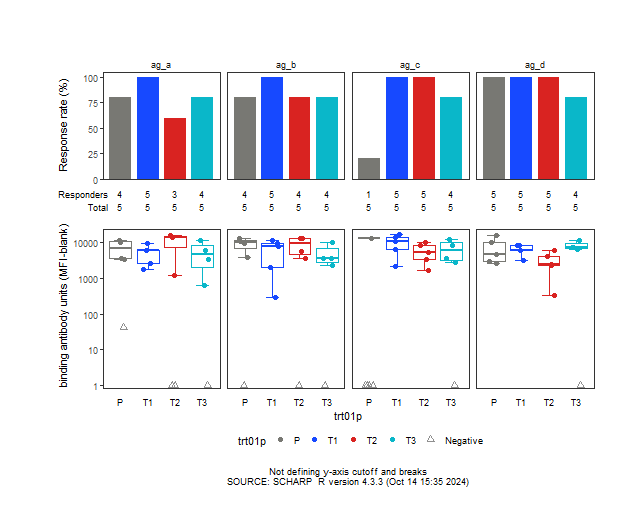
\includegraphics[width=8.75in,height=7.25in]{test_cases_files/figure-latex/unnamed-chunk-6-1} 

}

\caption[Figure 3.1 boxplot (pos. response boxplots)]{Figure 3.1 HVTN XYZ: IgA Response at Visit 5}\label{fig:unnamed-chunk-6-1}
\end{figure}
\clearpage\begin{figure}[H]

{\centering 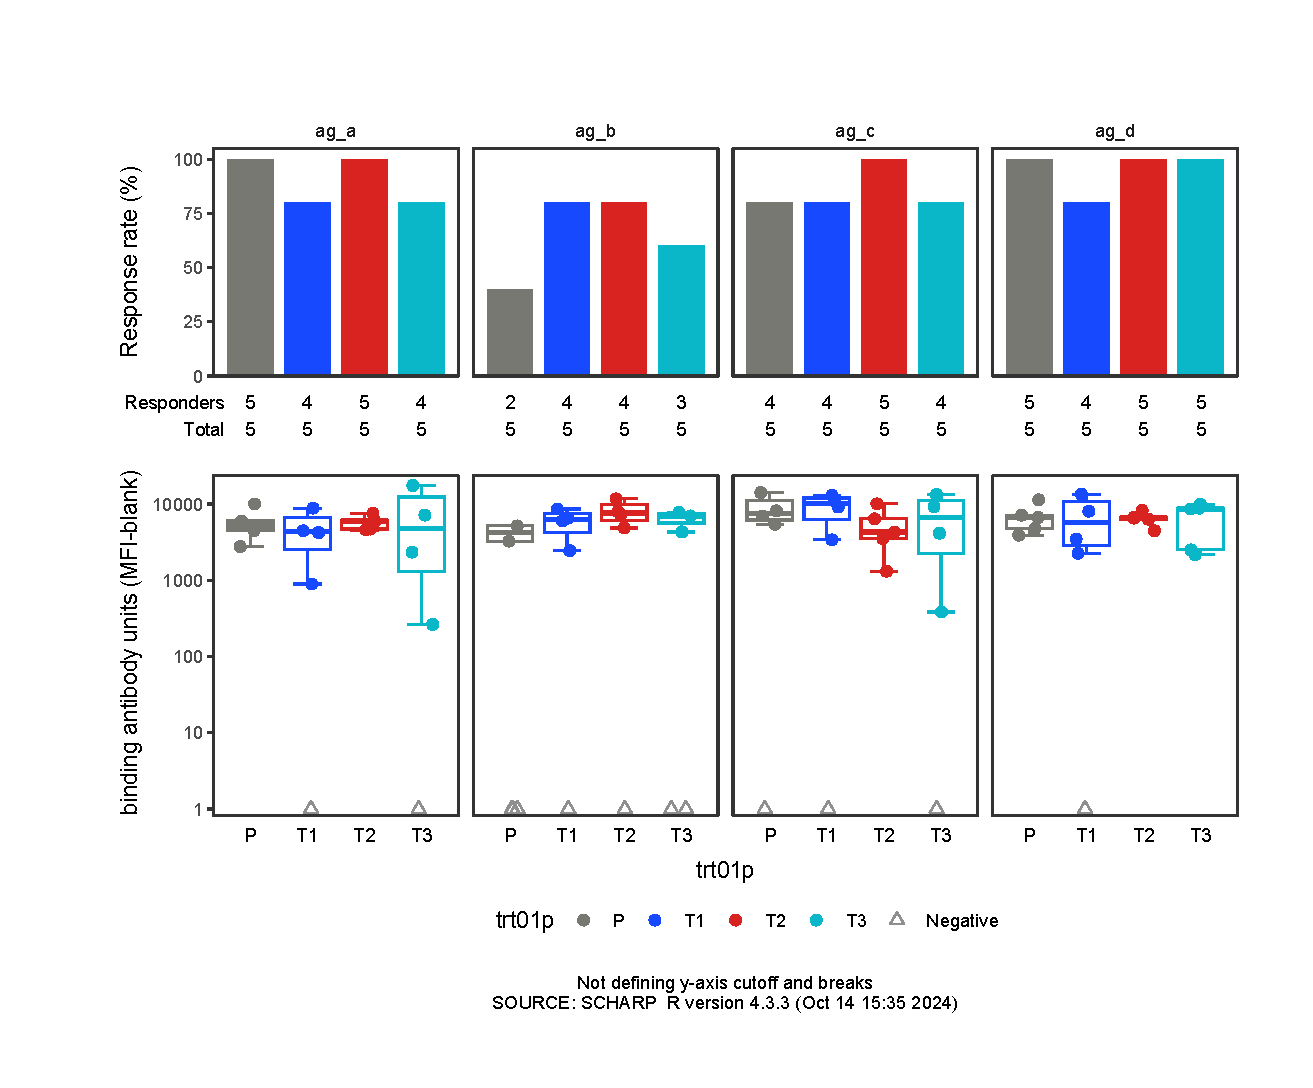
\includegraphics[width=8.75in,height=7.25in]{test_cases_files/figure-latex/unnamed-chunk-6-2} 

}

\caption[Figure 3.2 boxplot (pos. response boxplots)]{Figure 3.2 HVTN XYZ: IgA Response at Visit 7}\label{fig:unnamed-chunk-6-2}
\end{figure}
\clearpage\begin{figure}[H]

{\centering 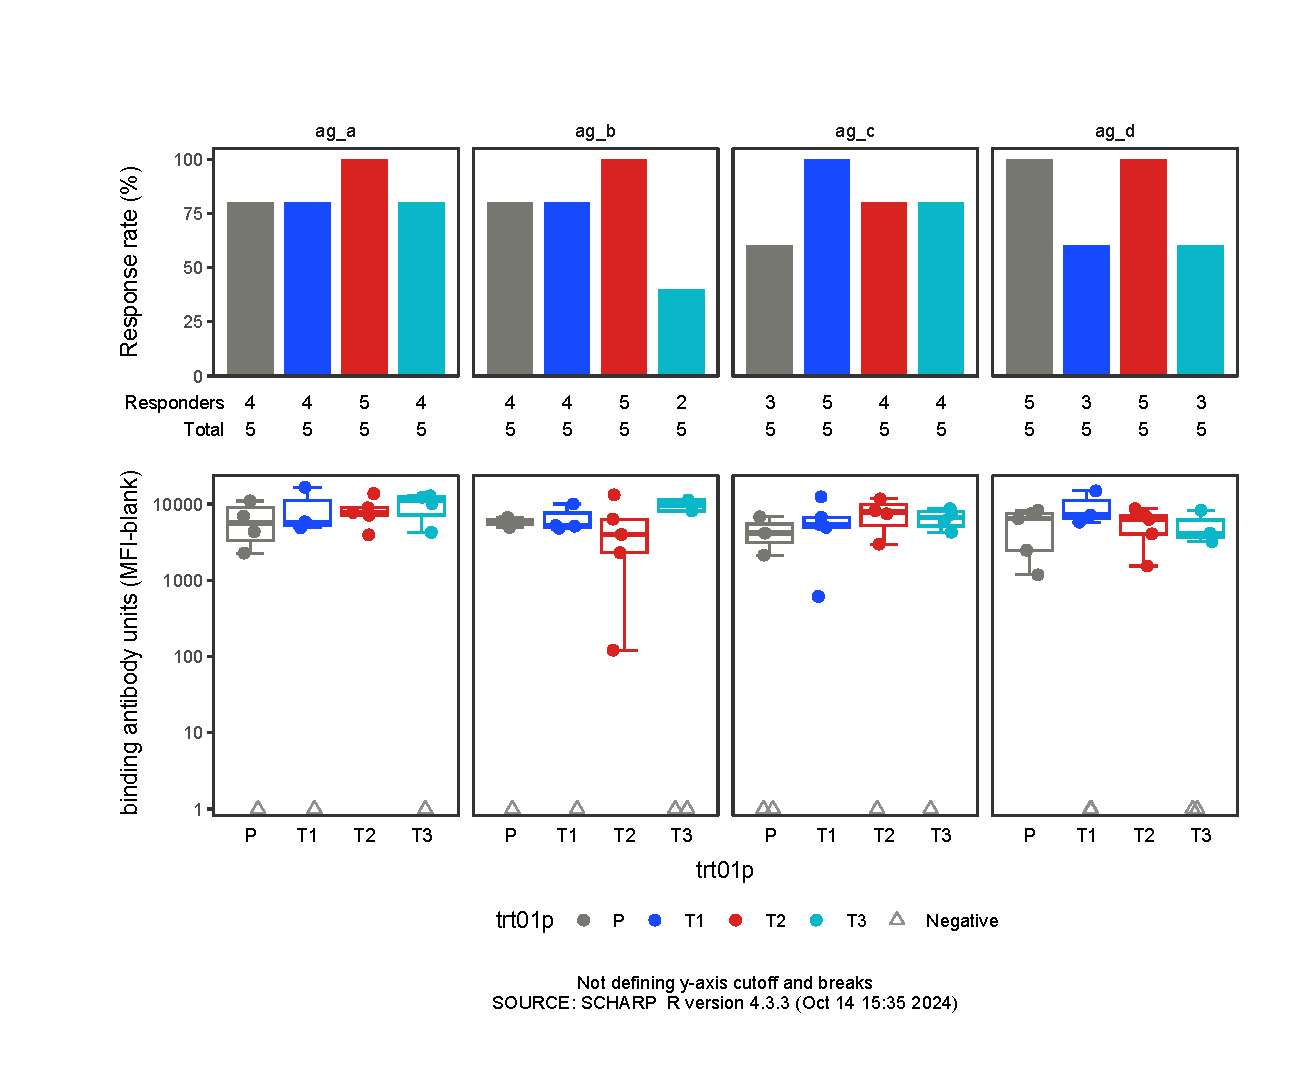
\includegraphics[width=8.75in,height=7.25in]{test_cases_files/figure-latex/unnamed-chunk-6-3} 

}

\caption[Figure 3.3 boxplot (pos. response boxplots)]{Figure 3.3 HVTN XYZ: IgA Response at Visit 11}\label{fig:unnamed-chunk-6-3}
\end{figure}
\clearpage

\begin{figure}[H]

{\centering 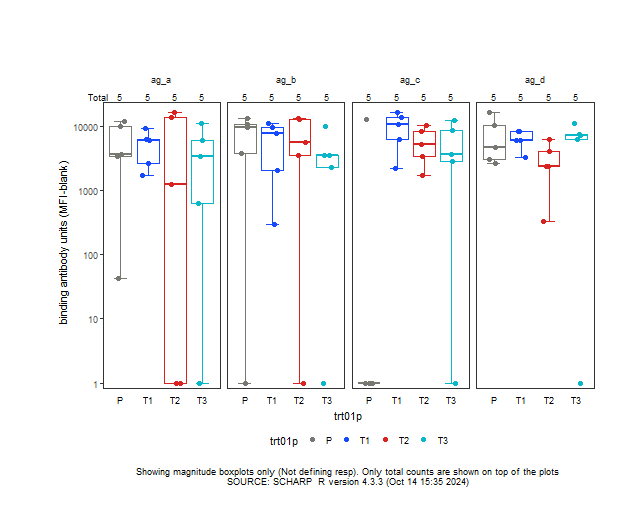
\includegraphics[width=8.75in,height=7.25in]{test_cases_files/figure-latex/unnamed-chunk-8-1} 

}

\caption[Figure 4.1 boxplot (pos. response boxplots)]{Figure 4.1 HVTN XYZ: IgA Response at Visit 5}\label{fig:unnamed-chunk-8}
\end{figure}
\clearpage

\begin{figure}[H]

{\centering 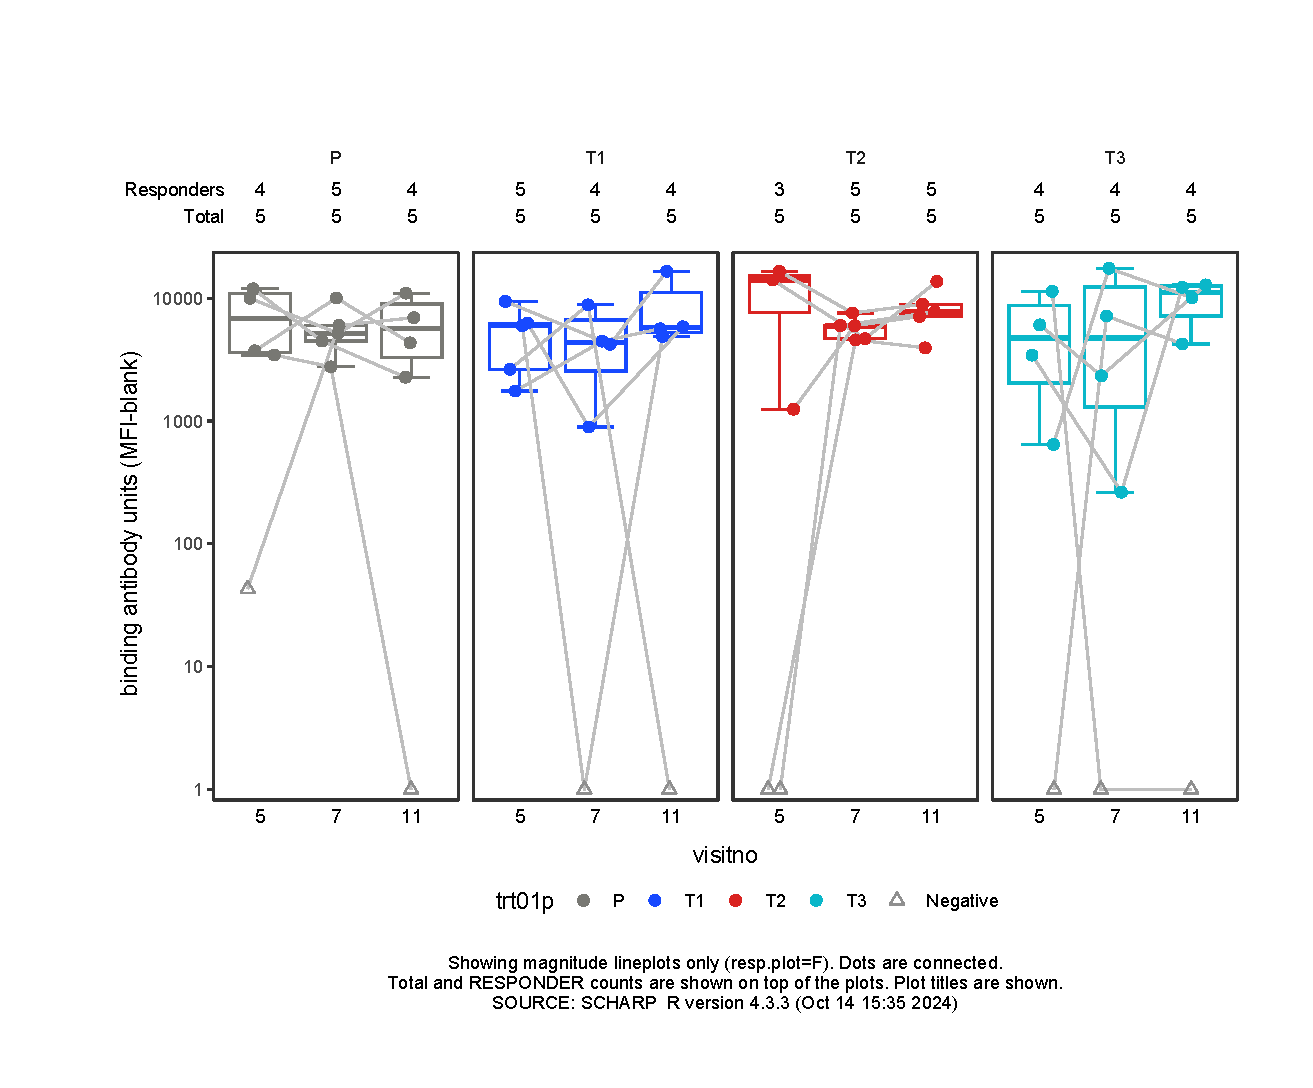
\includegraphics[width=8.75in,height=7.25in]{test_cases_files/figure-latex/unnamed-chunk-10-1} 

}

\caption[Figure 5.1 lineplot (pos. response boxplots)]{Figure 5.1 HVTN XYZ: IgA Response at Visit ag\_a}\label{fig:unnamed-chunk-10}
\end{figure}
\clearpage

\begin{figure}[H]

{\centering 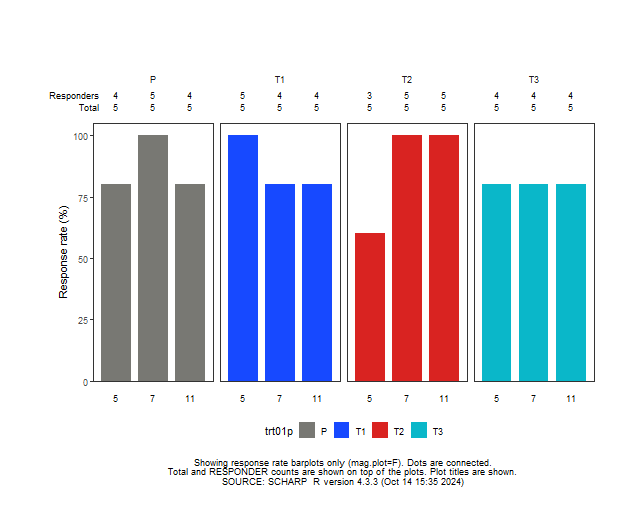
\includegraphics[width=8.75in,height=7.25in]{test_cases_files/figure-latex/unnamed-chunk-12-1} 

}

\caption[Figure 6.1 lineplot (pos. response boxplots)]{Figure 6.1 HVTN XYZ: IgA Response at Visit ag\_a}\label{fig:unnamed-chunk-12}
\end{figure}
\clearpage

\begin{figure}[H]

{\centering 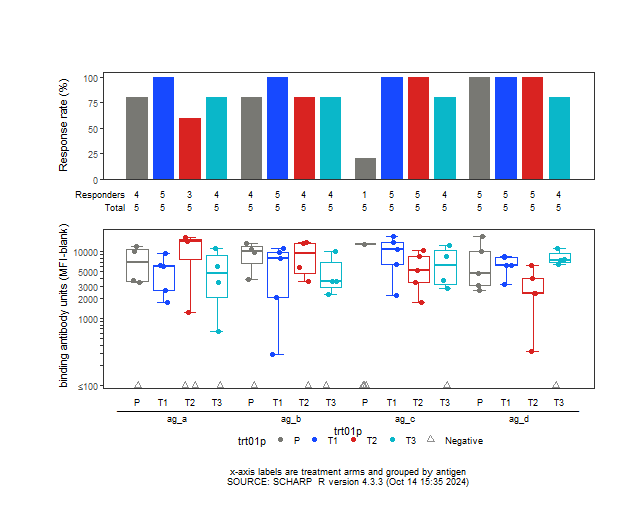
\includegraphics[width=8.75in,height=7.25in]{test_cases_files/figure-latex/unnamed-chunk-14-1} 

}

\caption[Figure 7.1 boxplot (pos. response boxplots)]{Figure 7.1 HVTN XYZ: IgA Response at Visit 5}\label{fig:unnamed-chunk-14}
\end{figure}
\clearpage

\begin{figure}[H]

{\centering 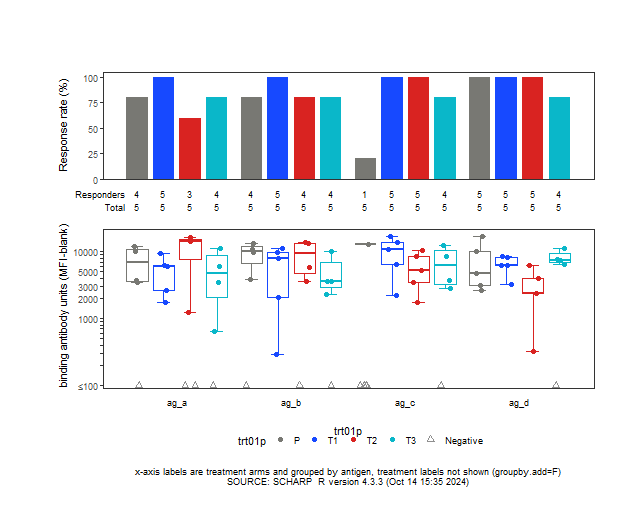
\includegraphics[width=8.75in,height=7.25in]{test_cases_files/figure-latex/unnamed-chunk-16-1} 

}

\caption[Figure 8.1 boxplot (pos. response boxplots)]{Figure 8.1 HVTN XYZ: IgA Response at Visit 5}\label{fig:unnamed-chunk-16}
\end{figure}
\clearpage

\begin{figure}[H]

{\centering 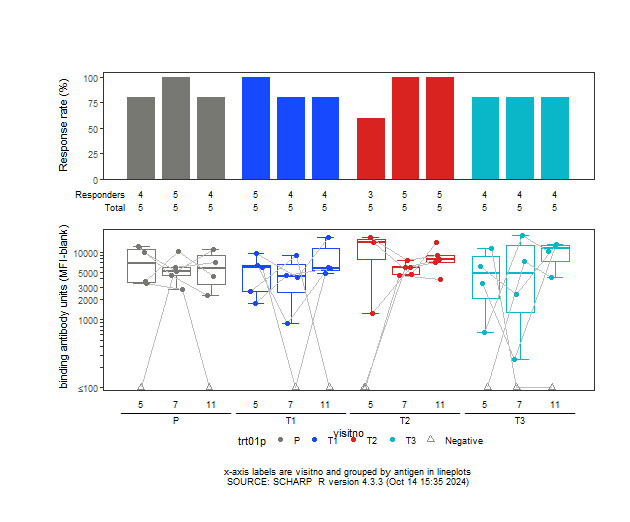
\includegraphics[width=8.75in,height=7.25in]{test_cases_files/figure-latex/unnamed-chunk-18-1} 

}

\caption[Figure 9.1 lineplot (pos. response boxplots)]{Figure 9.1 HVTN XYZ: IgA Response at Visit ag\_a}\label{fig:unnamed-chunk-18}
\end{figure}
\clearpage

\begin{figure}[H]

{\centering 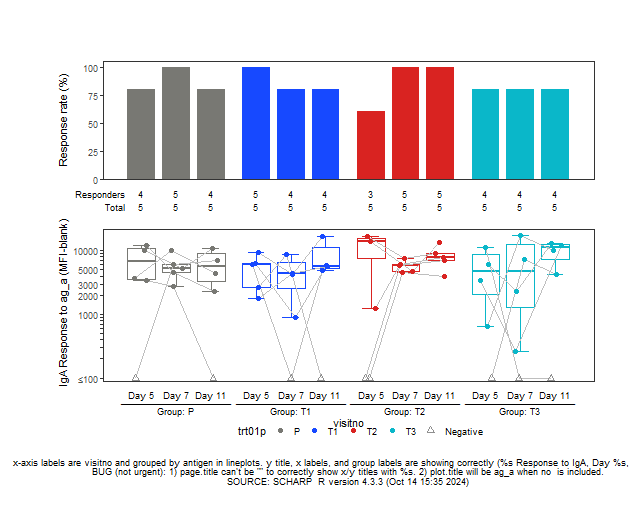
\includegraphics[width=8.75in,height=7.25in]{test_cases_files/figure-latex/unnamed-chunk-20-1} 

}

\caption[Figure 10.1 lineplot (pos. response boxplots)]{Figure 10.1 HVTN XYZ: IgA Response at Visit ag\_a}\label{fig:unnamed-chunk-20}
\end{figure}
\clearpage

\begin{figure}[H]

{\centering 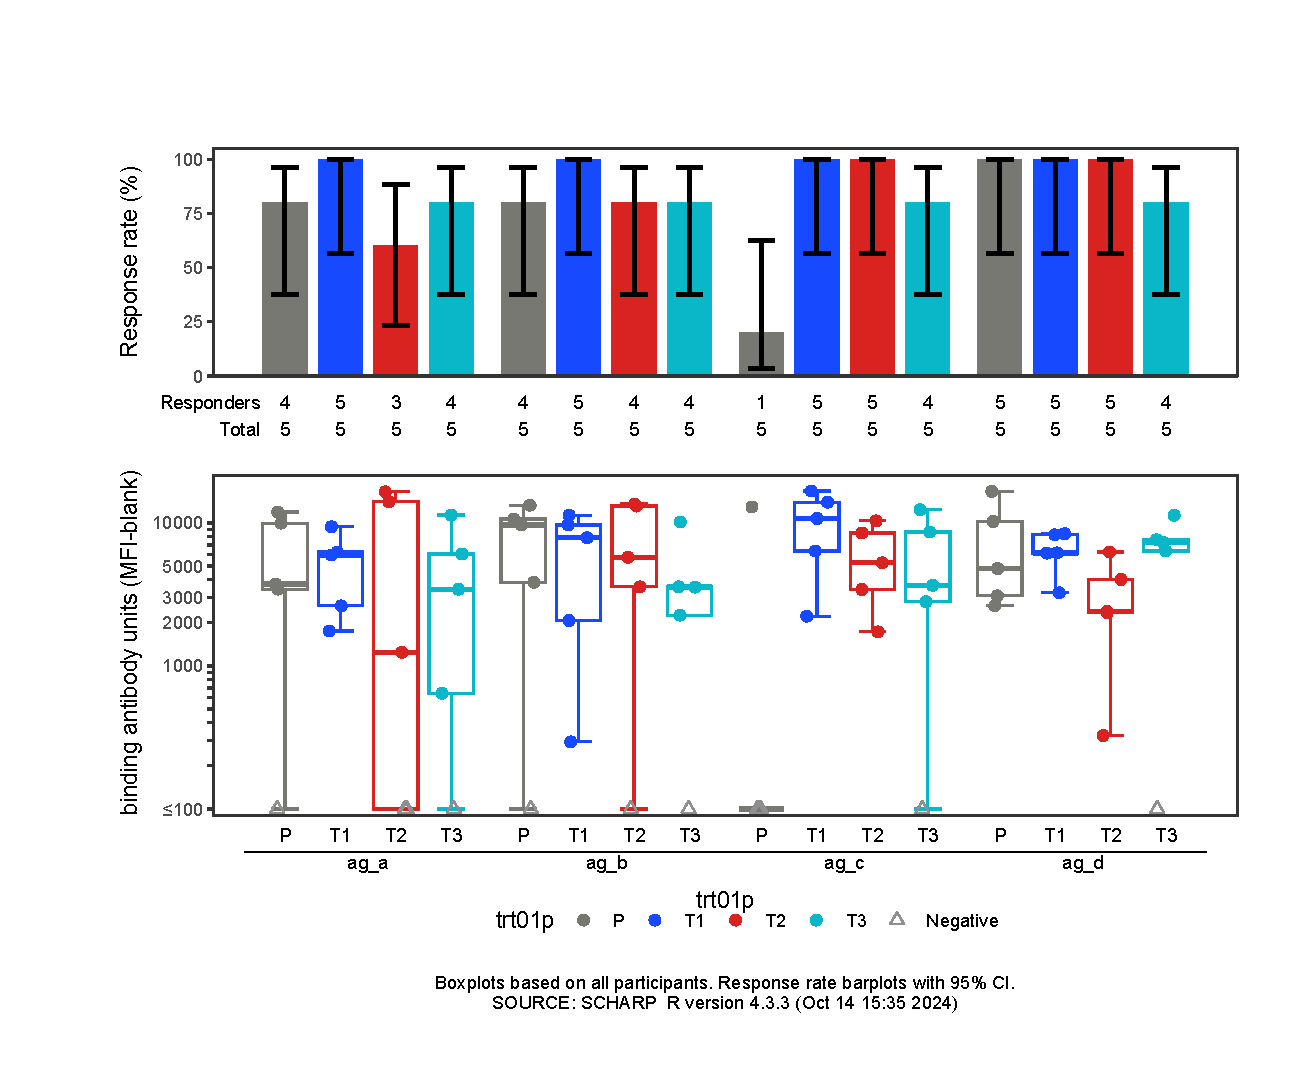
\includegraphics[width=8.75in,height=7.25in]{test_cases_files/figure-latex/unnamed-chunk-22-1} 

}

\caption[Figure 11.1 boxplot (pos. response boxplots)]{Figure 11.1 HVTN XYZ: IgA Response at Visit 5}\label{fig:unnamed-chunk-22}
\end{figure}
\clearpage

\begin{figure}[H]

{\centering 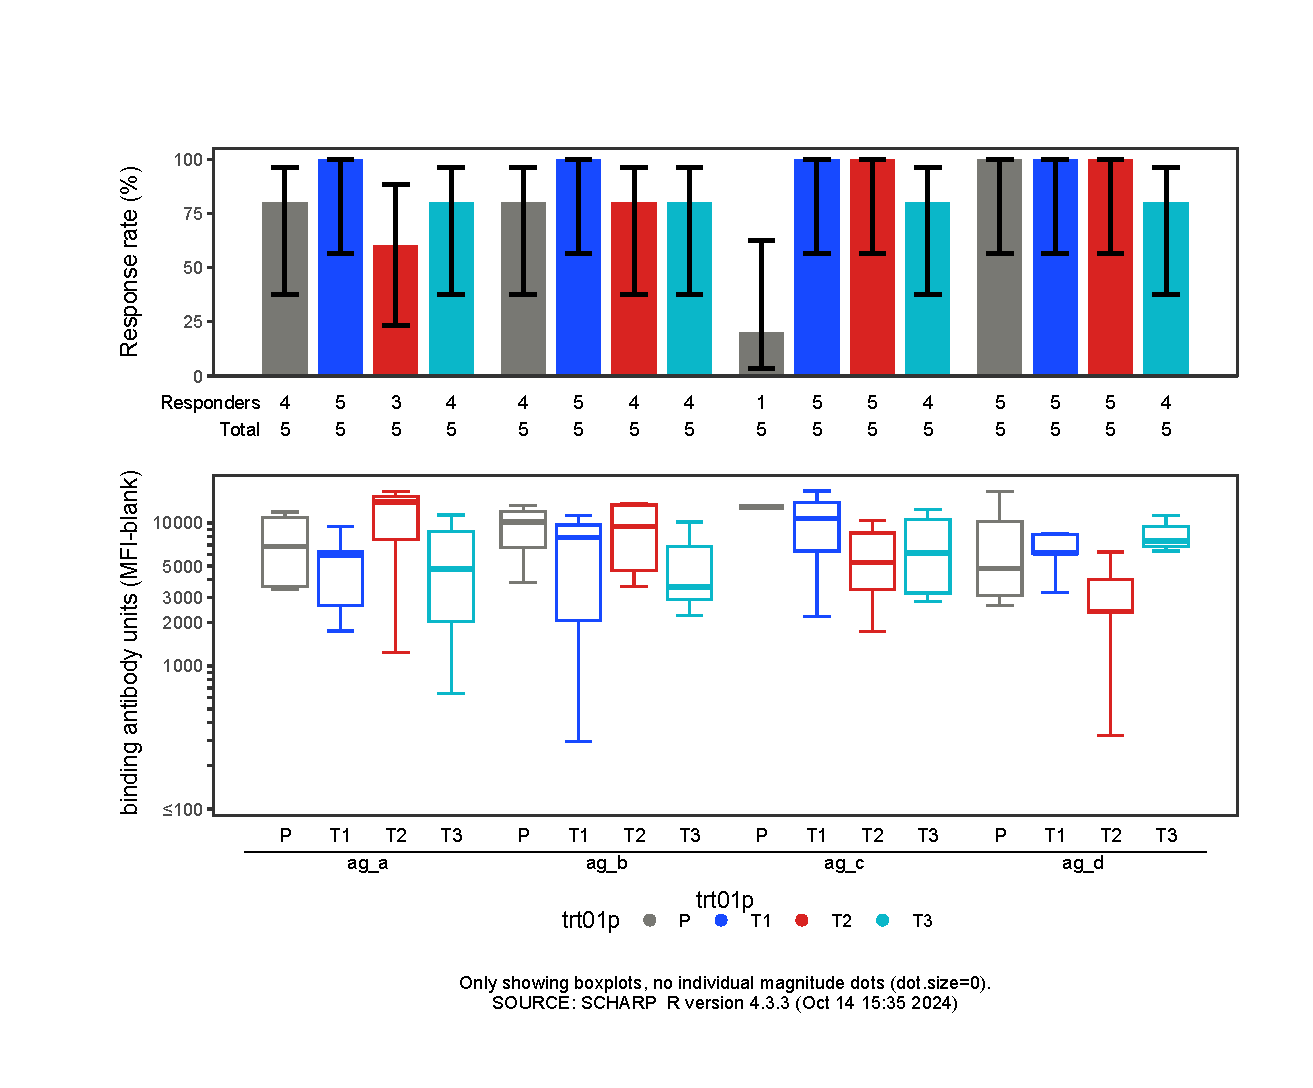
\includegraphics[width=8.75in,height=7.25in]{test_cases_files/figure-latex/unnamed-chunk-24-1} 

}

\caption[Figure 12.1 boxplot (pos. response boxplots)]{Figure 12.1 HVTN XYZ: IgA Response at Visit 5}\label{fig:unnamed-chunk-24}
\end{figure}
\clearpage

\begin{figure}[H]

{\centering 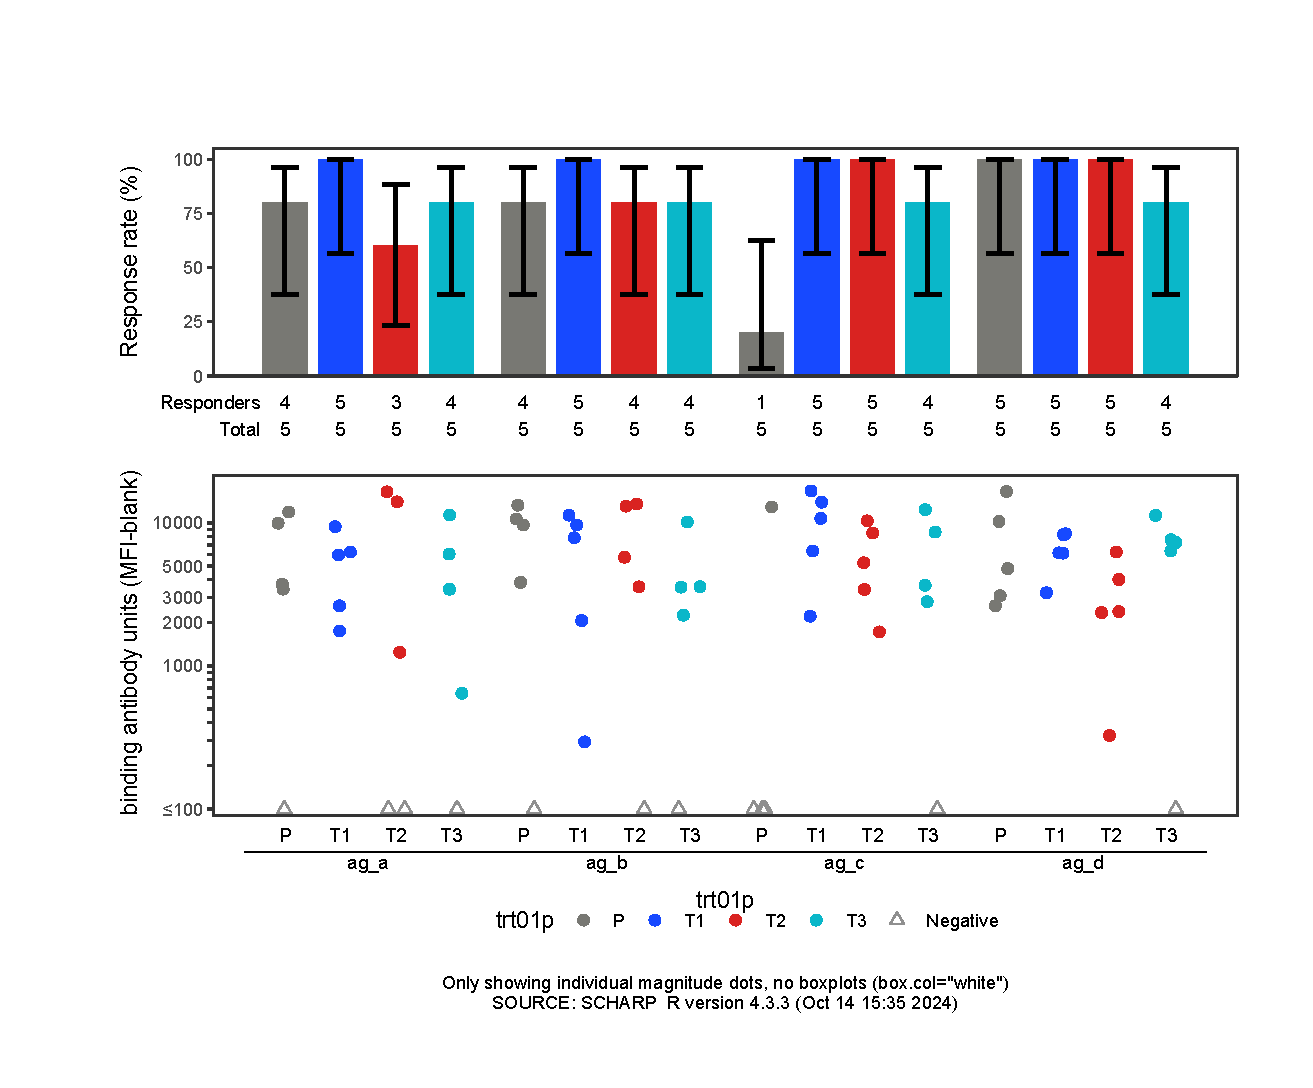
\includegraphics[width=8.75in,height=7.25in]{test_cases_files/figure-latex/unnamed-chunk-26-1} 

}

\caption[Figure 13.1 boxplot (pos. response boxplots)]{Figure 13.1 HVTN XYZ: IgA Response at Visit 5}\label{fig:unnamed-chunk-26}
\end{figure}
\clearpage

\begin{figure}[H]

{\centering 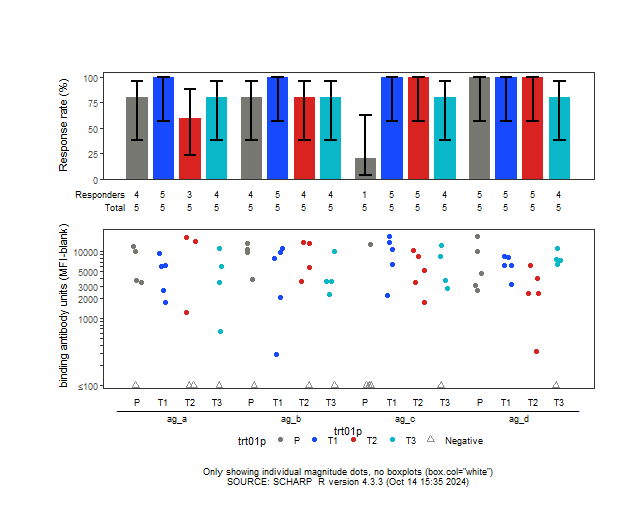
\includegraphics[width=8.75in,height=7.25in]{test_cases_files/figure-latex/unnamed-chunk-28-1} 

}

\caption[Figure 14.1 boxplot (pos. response boxplots)]{Figure 14.1 HVTN XYZ: IgA Response at Visit 5}\label{fig:unnamed-chunk-28}
\end{figure}
\clearpage

\begin{figure}[H]

{\centering 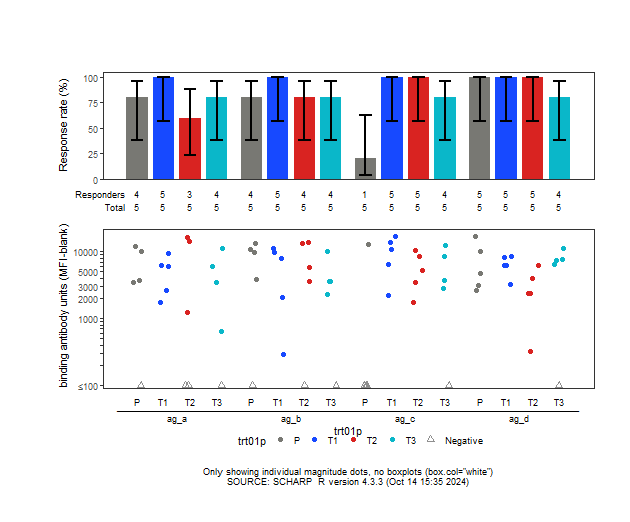
\includegraphics[width=8.75in,height=7.25in]{test_cases_files/figure-latex/unnamed-chunk-30-1} 

}

\caption[Figure 15.1 boxplot (pos. response boxplots)]{Figure 15.1 HVTN XYZ: IgA Response at Visit 5}\label{fig:unnamed-chunk-30}
\end{figure}
\clearpage

\begin{figure}[H]

{\centering 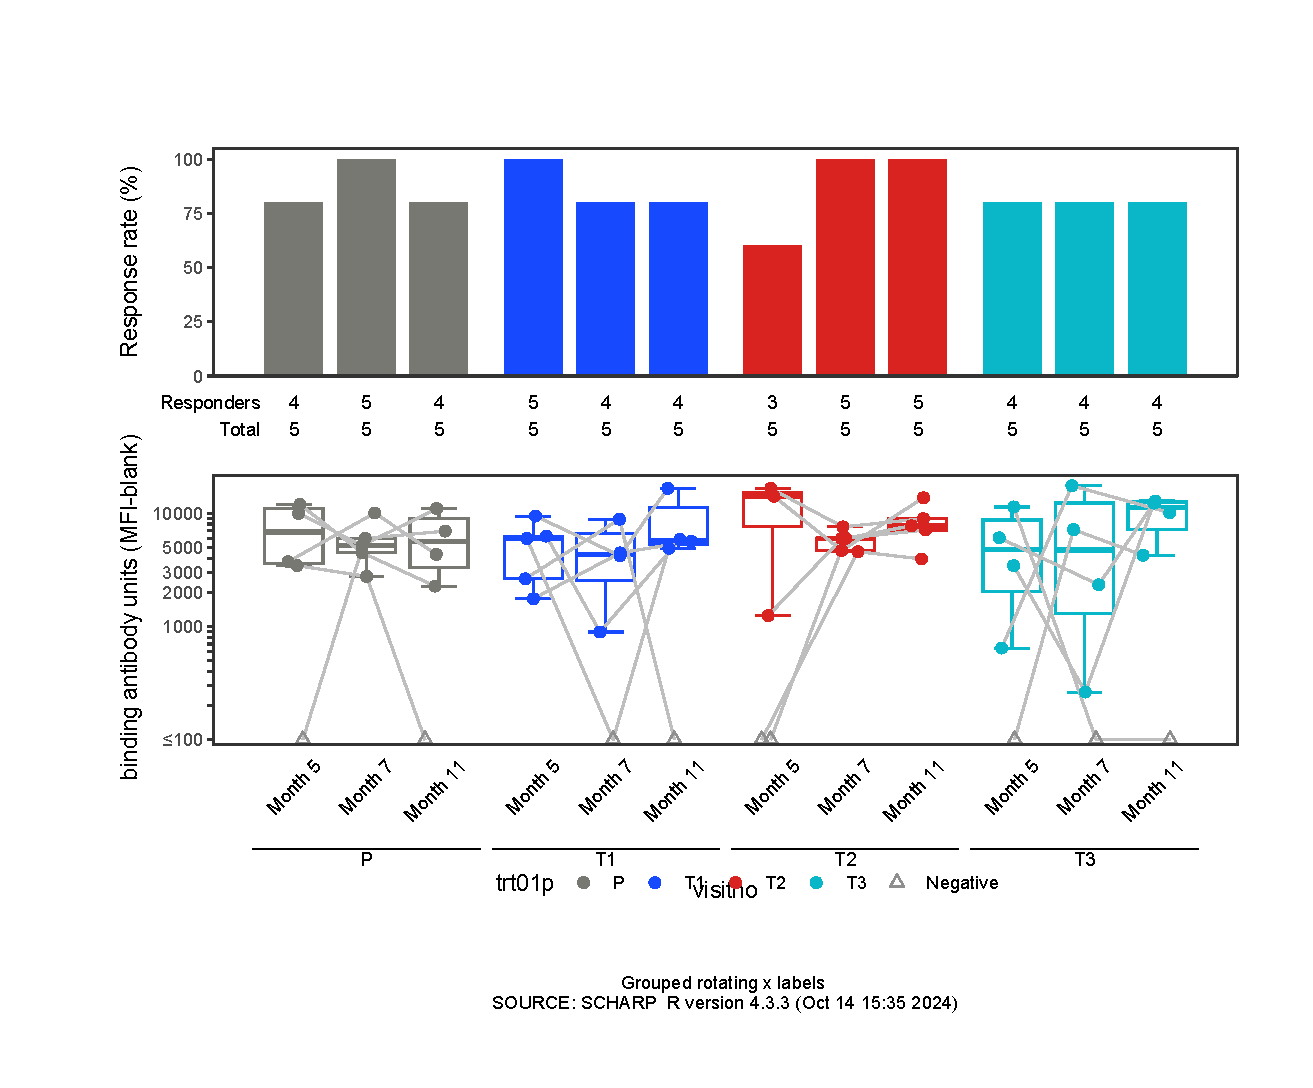
\includegraphics[width=8.75in,height=7.25in]{test_cases_files/figure-latex/unnamed-chunk-32-1} 

}

\caption[Figure 16.1 lineplot (pos. response boxplots)]{Figure 16.1 HVTN XYZ: IgA Response at Visit ag\_a}\label{fig:unnamed-chunk-32}
\end{figure}
\clearpage

\elandscape
\memoformat

\hypertarget{refs}{}
\begin{CSLReferences}{1}{0}
\leavevmode\vadjust pre{\hypertarget{ref-AgCo1998}{}}%
Agresti, Alan, and Brent A. Coull. 1998. {``Approximate Is Better Than
'Exact' for Interval Estimation of Binomial Proportions.''} \emph{The
American Statistician} 52: 119--26.

\leavevmode\vadjust pre{\hypertarget{ref-archary2016}{}}%
Archary, Derseree, Kelly E. Seaton, Jo-Ann S. Passmore, Lisa Werner, A
Deal, LJ Dunphy, Kelly B. Arnold, et al. 2016. {``Distinct Genital Tract
{HIV}-Specific Antibody Profiles Associated with Tenofovir Gel.''}
\emph{Mucosal Immunology} 9. \url{https://doi.org/10.1038/mi.2015.145}.

\leavevmode\vadjust pre{\hypertarget{ref-haynes_rv144_corr}{}}%
Haynes, Barton F., Peter B. Gilbert, M. Juliana McElrath, Susan
Zolla-Pazner, Georgia D. Tomaras, S. Munir Alam, David T. Evans, et al.
2012. {``Immune-Correlates Analysis of an {HIV-1} Vaccine Efficacy
Trial.''} \emph{New England Journal of Medicine} 366: 1275--86.

\leavevmode\vadjust pre{\hypertarget{ref-Huang2009-ao}{}}%
Huang, Yunda, Peter B. Gilbert, David C. Montefiori, and Steve G Self.
2009. {``Simultaneous Evaluation of the Magnitude and Breadth of a Left
and Right Censored Multivariate Response, with Application to {HIV}
Vaccine Development.''} \emph{Stat. Biopharm. Res.} 1 (1): 81--91.

\leavevmode\vadjust pre{\hypertarget{ref-seaton2014_vag_iga}{}}%
Seaton, Kelly E., Lamar Ballweber, Audrey Lan, Michele Donathan, Sean
Hughes, Lucia Vojtech, M. Anthony Moody, et al. 2014.
{``{HIV}s-1-Specific {IgA} Detected in Vaginal Secretions of {HIV}
Uninfected Women Participating in a Microbicide Trial in Southern Africa
Are Primarily Directed Toward Gp120 and Gp140 Specificities.''}
\emph{PloS One} 9 (7): e101863.
\url{https://journals.plos.org/plosone/article?id=10.1371/journal.pone.0101863}.

\leavevmode\vadjust pre{\hypertarget{ref-tomaras2008}{}}%
Tomaras, Georgia D., Nicole L. Yates, Pinghuang Liu, Li Qin, Genevieve
G. Fouda, Leslie L. Chavez, Allan C. deCamp, et al. 2008. {``Initial
b-Cell Responses to Transmitted Human Immunodeficiency Virus Type 1:
Virion-Binding Immunoglobulin m (IgM) and IgG Antibodies Followed by
Plasma Anti-{gp41} Antibodies with Ineffective Control of Initial
Viremia.''} \emph{Journal of Virology} 82 (24): 12449--63.

\leavevmode\vadjust pre{\hypertarget{ref-yates2018}{}}%
Yates, Nicole L., Allan C deCamp, Bette T Korber, Hua-Xin Liao, Carmela
Irene, Abraham Pinter, James Peacock, et al. 2018. {``{HIV}-1 Envelope
Glycoproteins from Diverse Clades Differentiate Antibody Responses and
Durability Among Vaccinees.''} Edited by Guido Silvestri. \emph{Journal
of Virology} 92 (8). \url{https://doi.org/10.1128/JVI.01843-17}.

\leavevmode\vadjust pre{\hypertarget{ref-yates_vaccine_induced_2014}{}}%
Yates, Nicole L., Hua-Xin Liao, Youyi Fong, Allan deCamp, Nathan A.
Vandergrift, William T. Williams, S. Munir Alam, et al. 2014.
{``Vaccine-Induced {Env} {V}1-{V}2 {IgG}3 Correlates with Lower {HIV-1}
Infection Risk and Declines Soon After Vaccination.''} \emph{Science
Translational Medicine} 6 (228): 228ra39--39.
\url{https://doi.org/10.1126/scitranslmed.3007730}.

\leavevmode\vadjust pre{\hypertarget{ref-yates2013}{}}%
Yates, Nicole L., Andrea R Stacey, Tracy L Nolen, Nathan A. Vandergrift,
M. Anthony Moody, David C. Montefiori, Kent J Weinhold, et al. 2013.
{``{HIV}-1 {gp41} Envelope {IgA} Is Frequently Elicited After
Transmission but Has an Initial Short Half-Life.''} \emph{Nature Mucosal
Immunology} 6 (4): 692--703.

\leavevmode\vadjust pre{\hypertarget{ref-zolla_pazner_2014}{}}%
Zolla-Pazner, Susan, Allan deCamp, Peter B. Gilbert, Constance Williams,
Nicole L. Yates, William T. Williams, Robert Howington, et al. 2014.
{``Vaccine-Induced {IgG} Antibodies to {V1V2} Regions of Multiple
{HIV-1} Subtypes Correlate with Decreased Risk of {HIV-1} Infection.''}
\emph{PloS One} 9 (2).
\url{https://journals.plos.org/plosone/article?id=10.1371/journal.pone.0087572}.

\end{CSLReferences}

\end{document}
